\documentclass[11pt,a4paper]{article}

\usepackage[a4paper,margin=1in]{geometry}
\usepackage[T1]{fontenc}
\usepackage[utf8]{inputenc}
\usepackage{lmodern}
\usepackage{setspace}
\usepackage{hyperref}
\usepackage{graphicx}

\setstretch{1.0}

\title{Software Development Report}
\author{Brandon MacGillivray}
\date{\today}

\begin{document}

\hypersetup{pageanchor=false}
\begin{titlepage}
\centering
{\LARGE Software Development Report\par}
\vspace{1.5cm}
{\large Project Title Placeholder\par}
\vspace{1cm}
{\large Brandon MacGillivray\par}
\vspace{0.5cm}
{\large Student ID Placeholder\par}
\vfill
{\large \today\par}
\end{titlepage}
\hypersetup{pageanchor=true}

\section*{Acknowledgements}

\tableofcontents
\newpage

\section{Introduction}

\section{Purpose, Operation and Validation}
\begin{itemize}
    \item What is the software intended to do?
    \item How does a user run or operate it?
    \item What inputs does it take and what outputs does it produce?
    \item How can the user tell it is working correctly?
    \item What evidence shows it performs its intended purpose?
\end{itemize}

The software is intended to implement and evaluate a lightweight 2D hand pose estimation pipeline for edge HCI, with a DRHand-inspired dual-branch model that predicts hand keypoints from RGB images and supports training, inference, benchmarking, and reproducible experiment reruns.

A user operates the software from the command line by setting up the documented Python environment, then running the repository scripts for the required workflow, such as \texttt{scripts/train.py} for training, \texttt{scripts/eval\_metrics.py} for checkpoint evaluation, and \texttt{scripts/predict\_image.py} for single-image inference, with inputs and options supplied as command-line arguments.

The software takes inputs such as dataset roots, checkpoint files, single RGB images, model and evaluation settings passed through command-line arguments, and it produces outputs such as trained checkpoint files, evaluation JSON metrics, aggregated CSV result tables, benchmark summaries, and qualitative prediction overlays or rendered figures.

A user can tell the software is working correctly when the lightweight test suite passes, the main command-line scripts load and print valid help output, and training, evaluation, inference, or benchmarking workflows execute successfully and produce outputs in the expected format that can be compared against the preserved reference JSON, CSV, checkpoint, and qualitative artefacts bundled in the repository.

\section{Design and Implementation}
\begin{itemize}
    \item How is the software designed overall?
    \item How is that design implemented in code?
    \item What are the main parts of the system and how do they work together?
\end{itemize}

The software is designed as a modular research artefact with a reusable Python package under \texttt{src/} for the core hand-pose pipeline, a set of command-line scripts under \texttt{scripts/} for running workflows such as training, evaluation, inference, and benchmarking, experiment definitions under \texttt{experiments/}, and curated documentation and preserved artefacts under \texttt{docs/}, allowing the same core implementation to support both development and reproducible assessment workflows.

The overall design is implemented as a structured Python package in which dataset handling is separated under \texttt{handpose.data}, model architecture and losses are defined under \texttt{handpose.models}, reusable training logic is kept under \texttt{handpose.training}, evaluation logic under \texttt{handpose.evaluation}, inference and fusion logic under \texttt{handpose.inference}, and checkpoint persistence under \texttt{handpose.checkpoints}, while thin command-line scripts call these modules to run complete workflows.

The main parts of the system are the dataset layer, the DRHand-inspired model, the inference and fusion layer, the training and evaluation pipelines, checkpoint management, and the command-line workflow scripts, and they work together by loading image and annotation data into a consistent format, passing that data through the model to generate heatmap and coordinate predictions, optionally fusing those predictions for final output, saving or loading checkpoints to preserve model state, and exposing these capabilities through scripts for training, evaluation, benchmarking, qualitative rendering, and single-image prediction.

\subsection{Significant Assumptions Made for the Design and Implementation}
\begin{itemize}
    \item What key assumptions were made when designing the software?
    \item How do those assumptions affect how the software works or is used?
\end{itemize}

Framework equivalence. The software assumes that the DRHand method can be reimplemented in PyTorch even though the original paper describes a TensorFlow implementation. As a result, this repository should be understood as a DRHand-inspired reconstruction rather than a strict reproduction, so exact numerical agreement with the original paper should not be expected.

Dataset substitution. The software assumes that the dual-branch DRHand idea can be studied meaningfully on RHD, HK26K / \texttt{coco\_hand}, and RH8 even though the original paper used YouTube2D Hands, GANerated Hands, STB, and RHD. This means the software evaluates the method under a different data regime, so its results support the reconstructed pipeline used in this project rather than the original paper’s exact benchmark setup.

Prepared input assumption. The software assumes that each input image already contains a clearly visible hand region and therefore does not implement a separate hand detector or crop-normalisation stage. This affects use because users must provide images or datasets where the hand is already reasonably framed, otherwise performance may degrade when the full image is simply resized to the network input size.

Fixed preprocessing strategy. The software assumes that full-image resize to 256 x 256 is an acceptable preprocessing strategy because the paper specifies the input size but does not define a more detailed input-normalisation pipeline. This makes the system simpler and easier to reproduce, but it also means the model is sensitive to changes in hand scale, position, and framing within the input image.

Coordinate representation. The software assumes that keypoints are represented internally as normalized (x, y) coordinates in the resized image space. This affects how the system works because training, inference, fusion, and evaluation all depend on this normalized representation, and conversion back to original pixel coordinates is only done when exporting predictions for human inspection or downstream use.

Heatmap supervision reconstruction. The software assumes Gaussian target heatmaps for heatmap regression because the paper defines an L2 heatmap loss but does not specify exactly how target heatmaps are constructed. This affects optimisation because the heatmap branch is trained to match smooth Gaussian peaks rather than some other target representation, which changes convergence behaviour and localisation sharpness.

Heatmap width assumption. The baseline system assumes \texttt{heatmap\_sigma = 2.0} because the original paper does not state a fixed Gaussian width. This matters because the spread of the target heatmap changes the difficulty and smoothness of the heatmap prediction task, so reproducing results depends on keeping this value consistent.

Wing-loss parameter assumption. The software assumes baseline Wing-loss values of w = 10.0 and epsilon = 2.0 because the paper gives the formula but not the actual parameter settings. This directly affects how the coordinate branch is trained, since different values change the relative penalty for small, medium, and large localisation errors.

Stage-2 optimisation assumption. The software assumes that stage 2 should jointly optimise both the heatmap and coordinate branches after the coordinate branch is added. This means the second training stage is not treated as coordinate-only fine-tuning, and the final model behaviour reflects continued interaction between both branches during optimisation.

Loss-weighting assumption. The baseline implementation assumes equal stage-2 loss weights for heatmap and coordinate supervision because the paper does not specify how the two losses should be balanced. This affects performance because the default behaviour gives both branches equal influence, while changing these weights shifts training emphasis toward one branch or the other.

Parameter update policy. The default implementation assumes that the backbone and heatmap branch remain trainable during stage 2 unless freezing is explicitly requested. This affects how the model learns because the full network can continue adapting in the second stage instead of treating stage-1 features as fixed.

Effective batch-size reconstruction. The software assumes that the paper’s stage-2 batch size of 256 can be approximated using batch size 64 with gradient accumulation on different hardware. This makes the training pipeline usable on more limited systems, but it also means the repository reproduces the paper’s intended effective batch size only approximately rather than literally.

Convergence assumption. The paper states that stage 1 runs until convergence and mentions 11 epochs in its original setup, but it does not define a complete stopping rule for this implementation context. The software therefore assumes a larger epoch budget together with early stopping, which means training duration is reconstructed pragmatically rather than copied exactly from the paper.

No explicit augmentation policy. The software assumes a simple deterministic preprocessing pipeline because the paper does not specify a detailed augmentation strategy. This improves clarity and reproducibility, but it also means robustness is achieved without relying on a strong augmentation regime unless a user adds one manually.

Single-hand target assumption. The software assumes one target hand per sample, selecting the requested or most visible hand where needed rather than jointly predicting multiple hands. This affects use because the repository is designed for single-hand pose estimation workflows rather than general multi-hand scene understanding.

Fusion threshold definition. The paper says fusion uses the median predicted knuckle length as the adaptive threshold alpha, but it does not fully formalise the exact skeleton edges in text. The implementation therefore assumes explicit edge lists for supported skeleton layouts, which means the behaviour of fusion depends partly on this code-level reconstruction.

Reduced 10-keypoint extension. The software assumes that the same overall DRHand-style architecture can be reused for a reduced 10-keypoint fingertip-and-base layout even though the original paper is written for 21 keypoints. This allows the project to test whether a smaller output space is sufficient for edge-HCI use, but it also means the reduced model is an adaptation introduced by this project rather than something directly defined in the paper.

Reduced-layout fusion assumption. Because the original paper does not define how fusion should work for a reduced keypoint layout, the implementation assumes a simplified edge set for the 10-keypoint model. This affects behaviour because the reduced fusion rule is a project-specific extension and therefore its outputs depend on an additional design decision beyond the original paper.

Visibility-aware evaluation assumption. The software assumes that evaluation should mask invisible joints when visibility information is available. This affects the reported metrics because performance is measured primarily on visible landmarks, which may differ from alternative evaluation protocols.

Reduced-layout EPE root assumption. The reduced shared-10 layout does not include the same root structure as the full 21-keypoint skeleton, so the implementation assumes an alternative root for root-relative EPE when necessary. This keeps EPE usable for reduced-layout experiments, but it means that reduced-layout EPE is not a perfectly identical measurement setup to the full-layout case.

\subsection{Languages, Packages, Frameworks, and Libraries Used}
\begin{itemize}
    \item What technologies were used to build the software?
    \item Why were these choices used in this project?
\end{itemize}

Python. The software was built primarily in Python because it provides a practical and widely used language for machine-learning research, rapid experimentation, data processing, and command-line workflow development. This made it suitable for implementing a research artefact that needed to support training, evaluation, inference, benchmarking, and reproducibility in a consistent codebase.

PyTorch. The main hand-pose pipeline was implemented in PyTorch because the project required a flexible deep-learning framework for defining custom model architectures, losses, and training procedures. PyTorch was particularly suitable for this DRHand-inspired implementation because it allowed the original dual-branch idea to be reconstructed clearly while remaining easy to debug and adapt for the reduced 10-keypoint and transfer-learning experiments.

Conda. A Conda-managed environment was used because the project depended on a mix of machine-learning, image-processing, and benchmarking packages that needed to be installed consistently across systems. Conda was chosen to reduce dependency conflicts and to make the installation and replication process more reliable for assessment.

NumPy. NumPy was used for numerical array processing because the software required lightweight handling of coordinates, image-derived data, and intermediate structured values outside the main tensor-training code. It was a natural choice because it integrates well with Python-based scientific and machine-learning workflows.

Pillow. Pillow was used for image loading and resizing because the project processes RGB hand images during training, evaluation, and inference. It was chosen as a simple and dependable library for image I/O and preprocessing without introducing unnecessary complexity.

MediaPipe. MediaPipe was used because the project included an explicit baseline comparison against a strong lightweight hand-tracking system and also relied on MediaPipe-related assets for pseudo-labelled or baseline-oriented workflows. This choice was important because it gave the project a practical reference point against a widely used real-time hand-pose system.

Matplotlib. Matplotlib was used for plotting and qualitative rendering because the project required visual inspection of predictions, generation of qualitative examples, and support for report-ready analysis figures. It was chosen because it is a standard and effective library for producing these outputs in Python.

PyTest. PyTest was used for automated testing because the repository needed a lightweight way to verify important behaviour such as model output shapes, fusion logic, and checkpoint validation. It was chosen to support software quality assurance and to provide a quick validation route for assessors and future users of the artefact.

psutil. The \texttt{psutil} package was used in benchmarking workflows because the project included deployment-oriented runtime analysis and needed process-level resource measurements in addition to model accuracy. It was chosen to support practical evaluation of the software on edge-oriented hardware settings.

\subsection{Overall Architecture / System Design and Interfaces Between Components}

\begin{figure}[htbp]
\centering
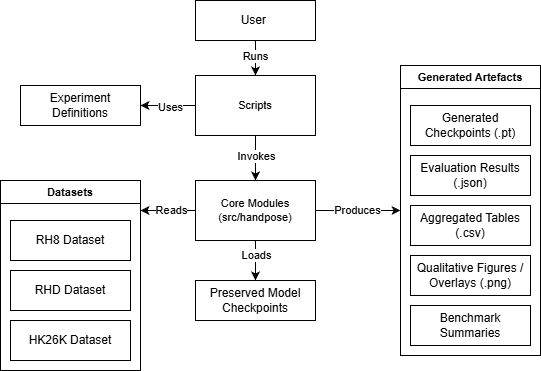
\includegraphics[width=0.6\textwidth]{4006_software_report-Page-2.drawio.png}
\caption{High-level architecture.}
\label{fig:software-architecture}
\end{figure}

\begin{figure}[htbp]
\centering
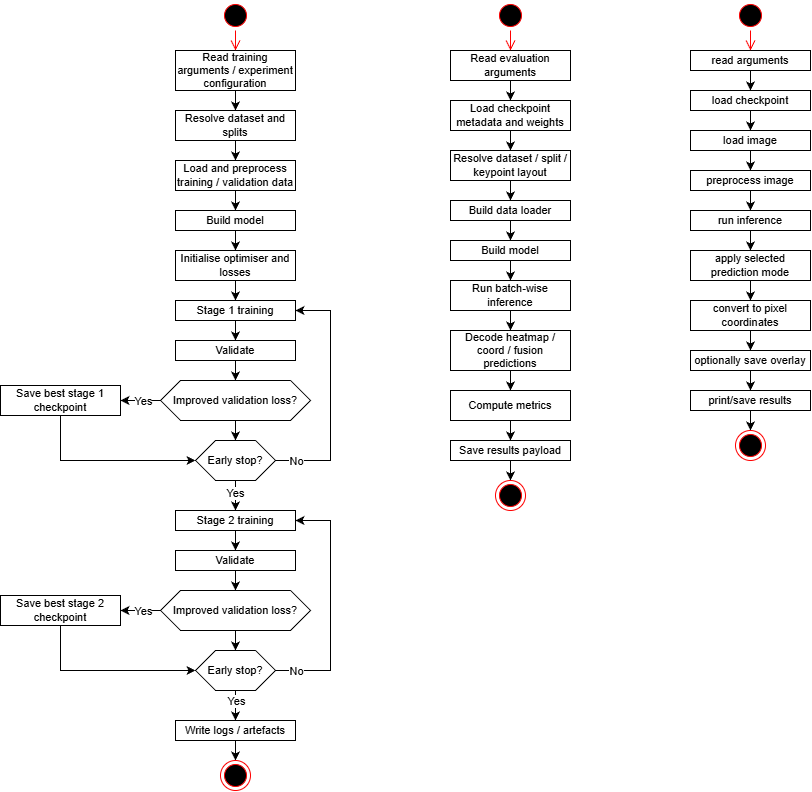
\includegraphics[width=1\textwidth,height=0.7\textheight,keepaspectratio]{4006_software_report-Page-4.drawio.png}
\caption{Training, evaluation and inference activity diagrams.}
\label{fig:training-evaluation-activities}
\end{figure}

\begin{itemize}
    \item What are the main components of the system?
    \item How do those components communicate with each other?
\end{itemize}

\subsection{Data Model(s), Including In-Memory Structures and Persistent Storage}
\begin{itemize}
    \item What data does the system store or process?
    \item How is that data represented in memory or saved persistently?
\end{itemize}

\subsection{Significant Methods, Functions, or Other Lower-Level Elements}
\begin{itemize}
    \item What lower-level parts of the implementation are most important?
    \item What does each important method or function do?
\end{itemize}

The most important lower-level implementation element is \texttt{HandPoseNet} in \texttt{src/handpose/models/hand\_pose\_model.py}, which acts as the main wrapper around the learned model. It combines the shared backbone, heatmap regression head, and coordinate regression head into one interface and provides the forward paths used during both training and inference. This makes it the central model component on which the rest of the repository depends.

At the architectural level, the most significant lower-level classes are \texttt{Backbone}, \texttt{Heatmap\_reg}, and \texttt{coord\_reg} in \texttt{src/handpose/models/architecture.py}, together with the reusable block definitions in \texttt{src/handpose/models/block.py}. These classes implement the shared feature extractor, the heatmap branch, the coordinate branch, and the depthwise-separable and upsampling building blocks from which the DRHand-inspired model is assembled.

The most important optimisation-related functions are \texttt{coords\_to\_heatmaps}, \texttt{HeatmapMSELoss}, and \texttt{WingLoss} in \texttt{src/handpose/models/losses.py}, along with \texttt{build\_optimizer\_stage1}, \texttt{build\_optimizer\_stage2}, \texttt{train\_one\_epoch}, and \texttt{validate} in the training modules. These functions define how supervision targets are constructed, how the two training losses are computed, how different stages of the model are optimised, and how batch-wise training and validation are carried out.

Another important group of lower-level functions appears in the preprocessing and dataset-loading code. The dataset factory and dataset classes in \texttt{src/handpose/data/} provide a unified interface for loading RHD and COCO-style hand datasets, while preprocessing helpers in \texttt{src/handpose/data/transforms.py} resize images, convert them to tensors, and rescale keypoint coordinates. These functions are significant because all training, evaluation, and inference workflows depend on the same shared input format.

The lower-level functions implementing branch fusion are also particularly important. In \texttt{src/handpose/inference/fusion.py}, functions such as \texttt{heatmaps\_to\_coords\_argmax}, \texttt{resolve\_fusion\_bone\_edges}, and \texttt{fuse\_coords} define how heatmap predictions are decoded and how the final fused prediction is selected from the heatmap and coordinate branches. These functions are central because the fusion rule is one of the defining design features of the implemented pipeline.

Checkpoint and evaluation handling are also key lower-level parts of the software. Functions in \texttt{src/handpose/checkpoints.py} define how checkpoints are validated, saved, and reloaded, while \texttt{evaluate\_checkpoint} in \texttt{src/handpose/evaluation/eval\_metrics\_core.py} performs the main metric computation for SSE, EPE, PCK, timing, and optional fusion diagnostics. These components are important because they make the repository reproducible and allow trained models to be reused consistently across training, inference, and result generation workflows.

Finally, the user-facing scripts under \texttt{scripts/} are thin but important workflow connectors. Scripts such as \texttt{train.py}, \texttt{eval\_metrics.py}, \texttt{predict\_image.py}, and \texttt{benchmark\_pipeline.py} do not contain the main modelling logic themselves, but they are the main entry points through which a user accesses the lower-level implementation for complete training, evaluation, inference, and benchmarking tasks.

\subsection{Important Errors and Their Conditions}
\begin{itemize}
    \item What important errors can occur?
    \item Under what conditions do those errors happen?
    \item How does the software respond to them?
\end{itemize}

Several important errors in the software are caused by invalid inputs, missing files, or inconsistent configuration between artefacts. For example, the checkpoint utilities raise errors when a checkpoint is missing required metadata fields, has a mismatched keypoint layout, contains duplicate keypoint indices, or uses an unsupported checkpoint version. Similar validation errors occur when invalid keypoint subsets are requested, when unsupported dataset names or split aliases are supplied, or when an invalid prediction mode or negative PCK threshold is passed on the command line. In these cases, the software responds by raising a clear \texttt{ValueError} and stopping execution rather than continuing with inconsistent state.

A second group of important errors occurs when required runtime resources are not available. Examples include missing dataset directories, missing image files, empty evaluation image folders, failed imports of optional dependencies such as MediaPipe, or requesting CUDA on a machine where it is not available. These conditions are handled through exceptions such as \texttt{FileNotFoundError} or \texttt{RuntimeError}. The software does not silently ignore these problems; instead, it fails early and reports the missing dependency, missing path, or unsupported device condition so that the user can correct the environment before rerunning the workflow.

Further errors can arise from invalid workflow state during training or evaluation. For example, stage-specific training functions raise errors if an unsupported stage number is used, if gradient accumulation is configured with an invalid value, or if stage 2 is requested without the required coordinate loss. Training also raises an error if \texttt{--skip-stage1} is used without providing an initial checkpoint. Evaluation and qualitative-rendering workflows can also fail when no samples match the requested dataset split or when the selected checkpoint does not contain the keypoints required for shared-10 evaluation or fusion. In these situations, the software again responds by terminating with an explicit error message, which helps prevent silent misuse of the repository and makes debugging more straightforward.


\subsection{User Interface Design}
\begin{itemize}
    \item How does the user interact with the software?
    \item What interface choices were made and why?
\end{itemize}

The user interacts with the software primarily through a command-line interface. The main workflows are exposed as separate Python scripts under \texttt{scripts/}, including training, evaluation, benchmarking, single-image inference, qualitative rendering, and result aggregation. In practice, the user runs these scripts from the repository root, supplies the required paths and options as command-line arguments, and receives outputs such as checkpoints, JSON result files, CSV summaries, printed metrics, or rendered visualisations.

This command-line design was chosen because the software is a research artefact rather than an end-user application. The main tasks involve running controlled experiments, reproducing reported results, evaluating checkpoints under different conditions, and generating analysis artefacts. These activities are better supported by explicit script arguments than by a graphical user interface, because command-line workflows are easier to document, automate, reproduce, and integrate with local machines, Conda environments, and HPC or Slurm-based execution.

Another important interface choice was to separate the reusable implementation from the user-facing entry points. The core logic is implemented in the \texttt{src/handpose/} package, while the scripts act as thin workflow wrappers around that logic. This was done so that the user interface remains simple at the script level while the lower-level code remains modular and reusable. As a result, users can run complete workflows through a small number of documented commands without needing to interact directly with the internal package structure.

The interface also relies on explicit file and path arguments for datasets, checkpoints, and output locations. This choice was made to keep the repository portable across different machines and storage layouts, especially since some datasets are external and not bundled with the artefact. By making these dependencies explicit at runtime, the software avoids hard-coding machine-specific paths and makes the execution process clearer for assessors and future users.

\subsection{Quality Assurance Steps}
\begin{itemize}
    \item What steps were taken to improve software quality?
    \item How was the software checked for correctness, reliability, and maintainability?
\end{itemize}

Several steps were taken to improve software quality throughout the project. The repository was organised into a modular structure, with reusable implementation code placed under \texttt{src/handpose/} and user-facing workflows exposed through separate scripts. This separation reduced duplication, made the system easier to understand, and improved maintainability by ensuring that training, evaluation, inference, and benchmarking all relied on shared core logic rather than separate ad hoc implementations.

Software quality was also improved through explicit validation and defensive error handling. Important interfaces such as checkpoint loading, dataset selection, prediction-mode resolution, keypoint-layout handling, and preprocessing inputs include checks that raise clear exceptions when invalid arguments or inconsistent artefacts are supplied. This helped reduce silent failure modes and made incorrect usage easier to identify and debug.

Correctness and reliability were checked using the lightweight automated test suite under \texttt{tests/}. These tests verify important repository contracts such as model output shapes, checkpoint schema validation, and fusion behaviour. In addition to automated tests, the repository also provides practical validation routes through documented commands in \texttt{INSTALL.md} and \texttt{REPLICATION\_GUIDE.md}, allowing the software to be checked by running real workflows and comparing regenerated outputs against preserved reference artefacts.

Maintainability was further supported through reproducibility-oriented documentation and artefact management. The repository includes installation instructions, requirement notes, a replication guide, curated experiment command files, preserved checkpoints, and saved result artefacts. These were important quality-assurance measures because they made the software easier to inspect, rerun, and extend, while also ensuring that the reported experimental outputs could be traced back to concrete workflows within the repository.


\subsubsection{Version Control and Versioning}
\begin{itemize}
    \item How was version control used during development?
    \item How were changes tracked and managed?
\end{itemize}

Version control was used throughout development by maintaining the project as a Git-based repository. This allowed the software, documentation, experiment definitions, and preserved artefacts to be developed within a single structured history rather than as disconnected files. Using version control was important because the project involved repeated changes to model design, training configuration, evaluation workflows, reporting artefacts, and supporting documentation, all of which needed to remain traceable over time.

Changes were tracked and managed through the normal Git workflow of recording edits to the repository as development progressed. This made it possible to monitor the evolution of scripts, source modules, experiment files, and paper materials, and helped prevent important changes from being lost or mixed together without record. It also supported safer experimentation, since alternative implementations or revised configurations could be introduced while preserving the earlier state of the project.

\subsubsection{Code Style and Convention}
\begin{itemize}
    \item What code style or conventions were followed?
    \item How did those conventions help keep the code clear and consistent?
\end{itemize}

The code follows a consistent Python style based on clear module separation, descriptive function names, and lightweight internal documentation. The repository is organised by responsibility, with separate modules for data loading, model definition, training, inference, evaluation, and checkpoint handling. Within these modules, functions and classes generally use descriptive snake\_case naming for functions and variables, and class-based naming for model components such as \texttt{HandPoseNet}. This made the code easier to navigate because related logic was grouped together rather than scattered across large scripts.

A consistent convention was also followed for docstrings and purpose statements. Most modules begin with a short summary docstring explaining their role in the repository, and most important functions include concise docstrings describing what they do. This helped keep the code clear because users and future readers can understand the role of a file or function without having to infer it entirely from implementation details.

The code also follows a convention of keeping user-facing workflow logic separate from reusable implementation logic. Scripts under \texttt{scripts/} mainly parse arguments and call functions from the \texttt{src/handpose/} package, while the package itself contains the lower-level logic. This convention improved consistency because training, evaluation, inference, and benchmarking were all built on shared internal code rather than separate duplicated implementations.

Another important convention is the use of explicit validation and informative error messages at key interfaces. Functions that depend on specific assumptions, such as checkpoint schema, prediction modes, dataset names, keypoint layouts, or device availability, usually check these conditions directly and raise clear exceptions if they are violated. This kept the behaviour of the software more predictable and made the codebase easier to maintain, since failures tended to occur close to the source of the problem rather than emerging later as ambiguous downstream bugs.

Finally, the repository shows a consistent testing convention in which small focused tests are used to protect important contracts such as model output shapes, checkpoint validation, and fusion behaviour. This helped reinforce code clarity and consistency because the expected behaviour of core components was made explicit both in implementation and in accompanying tests.


\subsubsection{Automated Testing}
\begin{itemize}
    \item What automated tests were implemented?
    \item What parts of the software do those tests verify?
\end{itemize}

The repository includes a lightweight automated test suite implemented with \texttt{pytest}. The tests are intended as a fast validation layer that checks a small number of important software contracts before running more expensive workflows such as full training or dataset-based evaluation. This makes them useful both during development and as a first confidence check for assessors or future users of the repository.

One group of tests verifies model-shape behaviour. In \texttt{tests/test\_model\_shapes.py}, the test suite checks that \texttt{HandPoseNet} produces outputs of the expected shape for both the standard 21-keypoint configuration and the reduced 10-keypoint configuration. These tests verify that the model returns heatmaps of shape \texttt{(N, K, 64, 64)} and coordinate outputs of shape \texttt{(N, K, 2)}, and also confirm that these outputs remain finite. This protects the most basic interface contract of the learned model.

A second group of tests verifies the fusion-related helper functions. In \texttt{tests/test\_fusion.py}, the software checks that heatmap argmax decoding returns the expected normalized coordinates, that the standard 21-joint fusion edge definition is resolved correctly, and that the reduced tip-and-base 10-joint layout is handled correctly while unsupported layouts are rejected. These tests verify the correctness of important lower-level logic used in fused inference.

A third group of tests verifies checkpoint schema handling. In \texttt{tests/test\_checkpoints.py}, the suite checks that valid checkpoints are accepted and normalized correctly, while malformed checkpoints with duplicate keypoint indices or inconsistent keypoint metadata are rejected. These tests verify the repository's checkpoint contract, which is important because the same checkpoint format is used across training, evaluation, inference, and preserved artefact reuse.

Finally, the \texttt{tests/conftest.py} configuration ensures that the \texttt{src/} tree is importable when tests are run from the repository root. This supports the automated test workflow by making the repository package available consistently during test execution. Overall, the automated tests focus on core structural correctness rather than full end-to-end experiment reproduction, while the latter is handled through the documented validation and replication commands elsewhere in the repository.

\appendix

\section{Appendices}

\end{document}
